% CORN — simplified architecture flow chart
% Compile with: pdflatex architecture-flowchart-simple.tex
% (uses TikZ; no external assets required)

\documentclass[border=10pt]{standalone}

\usepackage{tikz}
\usepackage{helvet}
\renewcommand{\familydefault}{\sfdefault}

\usetikzlibrary{positioning,arrows.meta,calc,shapes.geometric}

\begin{document}
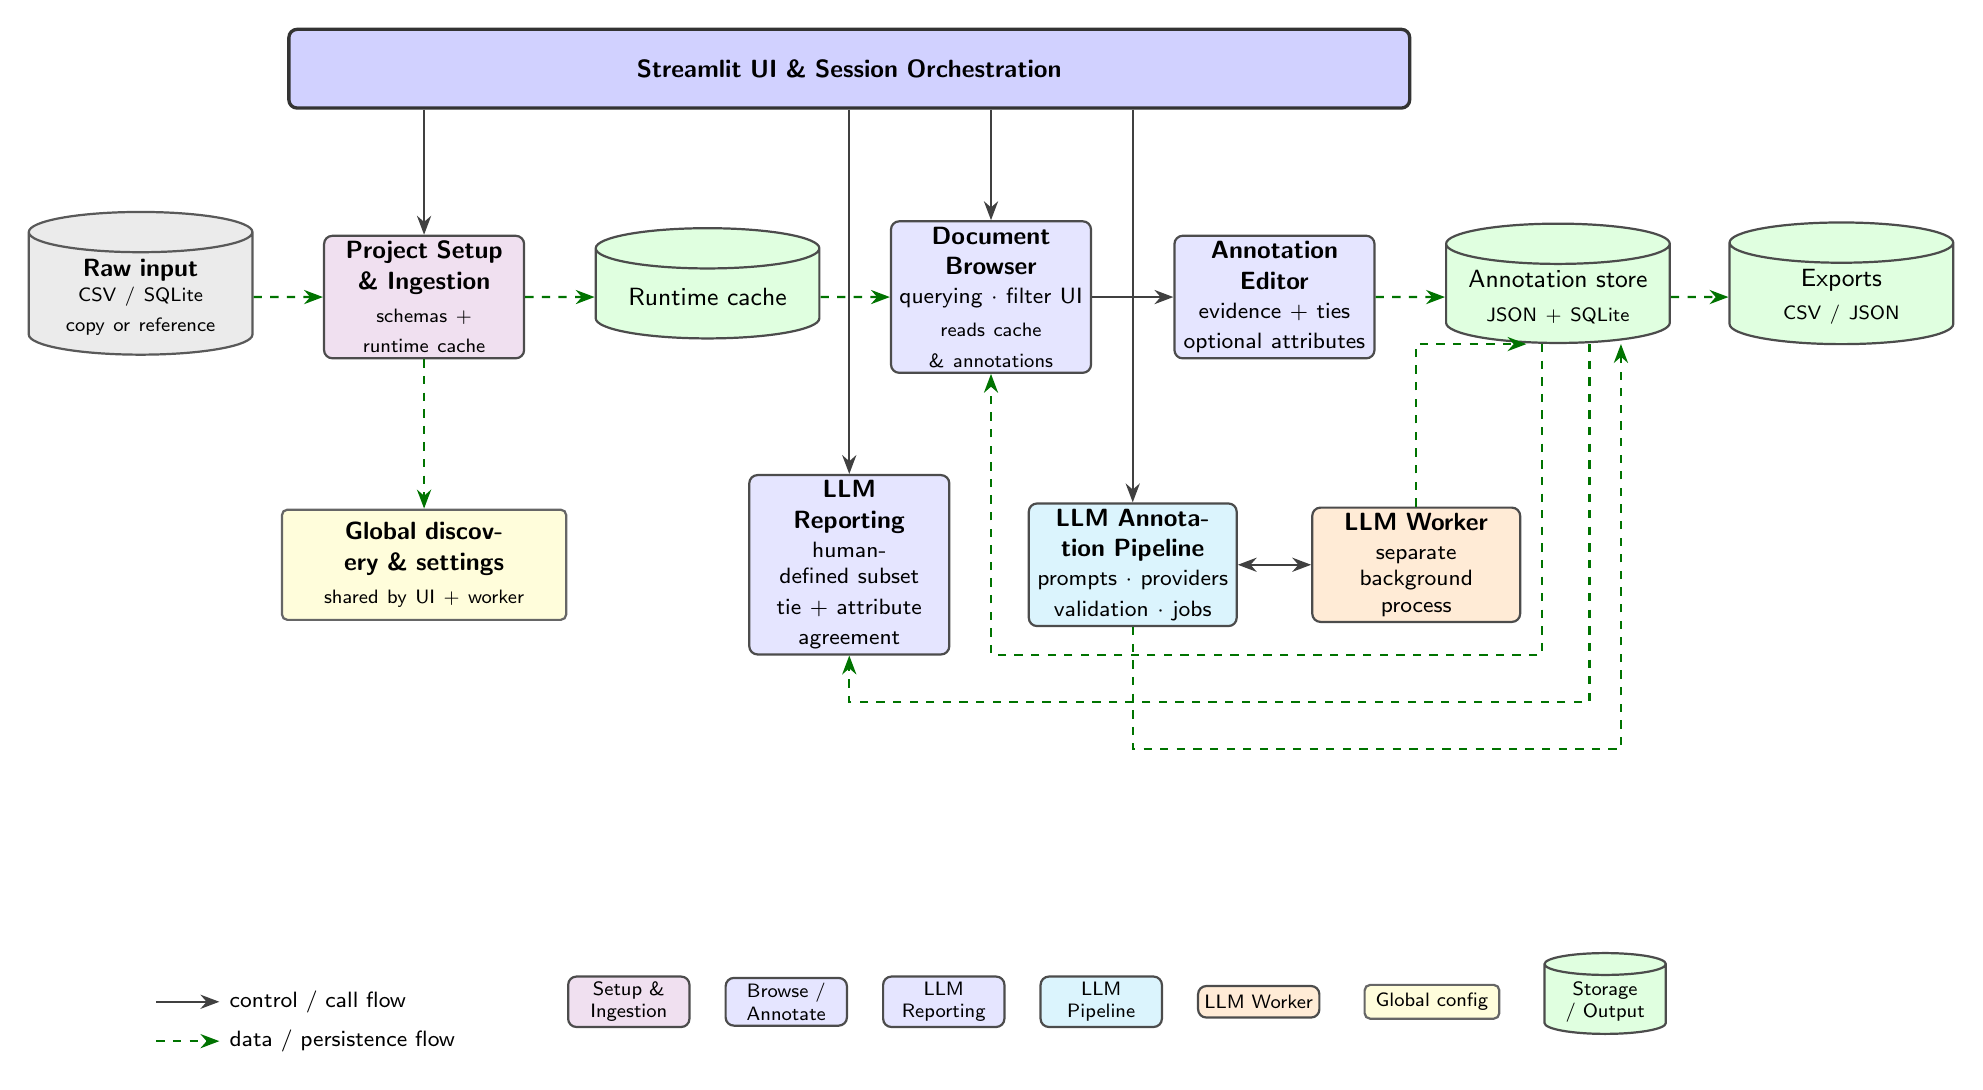
\begin{tikzpicture}[
    font=\small,
    >={Stealth[length=2.4mm]},
    x=1cm, y=1cm,
    % --- node styles -------------------------------------------------
    raw/.style={
        cylinder, shape border rotate=90, aspect=0.18,
        draw=black!65, thick, fill=black!8, align=center,
        text width=27mm, minimum height=14mm, inner sep=2pt},
    setup/.style={
        rectangle, rounded corners=3pt, draw=black!70, thick,
        fill=violet!12, align=center, text width=24mm,
        minimum height=12mm, inner sep=2pt},
    core/.style={
        rectangle, rounded corners=3pt, draw=black!70, thick,
        fill=blue!10, align=center, text width=24mm,
        minimum height=12mm, inner sep=2pt},
    llm/.style={
        rectangle, rounded corners=3pt, draw=black!70, thick,
        fill=cyan!14, align=center, text width=25mm,
        minimum height=13mm, inner sep=2pt},
    worker/.style={
        rectangle, rounded corners=3pt, draw=black!70, thick,
        fill=orange!16, align=center, text width=25mm,
        minimum height=13mm, inner sep=2pt},
    store/.style={
        cylinder, shape border rotate=90, aspect=0.18,
        draw=black!70, thick, fill=green!12, align=center,
        text width=27mm, minimum height=14mm, inner sep=2pt},
    gstore/.style={
        rectangle, rounded corners=2pt, draw=black!60, thick,
        fill=yellow!14, align=center, text width=34mm,
        minimum height=14mm, inner sep=3pt},
    orchestrator/.style={
        rectangle, rounded corners=3pt, draw=black!80, very thick,
        fill=blue!18, align=center, text width=140mm,
        minimum height=10mm},
    % --- edge styles -------------------------------------------------
    flow/.style={->, thick, black!75},
    flowbi/.style={<->, thick, black!75},
    dataflow/.style={->, thick, green!45!black, dashed}
]

% ======================================================================
%  Main data-flow chain (left -> right), row y = 0
% ======================================================================
\node[raw]   (raw)       at ( 0.0, 0) {\textbf{Raw input}\\[1pt]\scriptsize CSV / SQLite\\ copy or reference};
\node[setup] (setup)     at ( 3.6, 0) {\textbf{Project Setup}\\\textbf{\& Ingestion}\\[1pt]\scriptsize schemas + runtime cache};
\node[store] (runtimedb) at ( 7.2, 0) {Runtime cache\\[1pt]};
\node[core]  (browser)   at (10.8, 0) {\textbf{Document}\\\textbf{Browser}\\[1pt]\footnotesize querying $\cdot$ filter UI\\[1pt]\scriptsize reads cache \& annotations};
\node[core]  (editor)    at (14.4, 0) {\textbf{Annotation}\\\textbf{Editor}\\[1pt]\footnotesize evidence + ties\\ optional attributes};
\node[store] (annstore)  at (18.0, 0) {Annotation store\\[1pt]\scriptsize JSON + SQLite};
\node[store] (exports)   at (21.6, 0) {Exports\\[1pt]\scriptsize CSV / JSON};

% ======================================================================
%  Orchestrator (top), spanning setup .. editor
% ======================================================================
\node[orchestrator] (ui) at (9.0, 2.9)
    {\textbf{Streamlit UI \& Session Orchestration}};

% ======================================================================
%  LLM branch (below main row), y = -3.3
% ======================================================================
\node[core]   (reporting) at ( 9.0, -3.4)
    {\textbf{LLM}\\\textbf{Reporting}\\[1pt]\footnotesize human-defined subset\\ tie + attribute agreement};
\node[llm]    (pipeline) at (12.6, -3.4)
    {\textbf{LLM Annotation Pipeline}\\[1pt]\footnotesize prompts $\cdot$ providers\\ validation $\cdot$ jobs};
\node[worker] (worker)   at (16.2, -3.4)
    {\textbf{LLM Worker}\\[1pt]\footnotesize separate background\\ process\\ };

% global, app-wide artifacts (registry + provider settings)
\node[gstore] (global) at (3.6, -3.4)
    {\textbf{Global discovery \& settings}\\[1pt]\scriptsize shared by UI + worker};

% ======================================================================
%  Control / call flow (solid) — orchestrator drops straight down
% ======================================================================
\draw[flow] (ui.south -| setup.north)    -- (setup.north);
\draw[flow] (ui.south -| browser.north)  -- (browser.north);
\draw[flow] (ui.south -| reporting.north) -- (reporting.north);
\draw[flow] (ui.south -| pipeline.north) -- (pipeline.north);   % vertical in browser/editor gap
\draw[flow] (browser) -- (editor);                              % in-app workflow

% pipeline <-> worker
\draw[flowbi] (pipeline) -- (worker);

% ======================================================================
%  Data / persistence flow (dashed)
% ======================================================================
\draw[dataflow] (raw)       -- (setup);                 % source data in
\draw[dataflow] (setup)     -- (runtimedb);             % build cache
\draw[dataflow] (runtimedb) -- (browser);               % read for queries
\draw[dataflow] (editor)    -- (annstore);              % persist annotations
\draw[dataflow] (annstore)  -- (exports);               % export
\draw[dataflow] (setup.south) -- (global.north);        % registers project + config

% browser ALSO reads the annotation store (annotation presence + LLM coverage
% filters); routed through a lane pinned below pipeline.south so it clears the
% LLM node regardless of how tall its text makes it.
\coordinate (laneBrowser) at ($(pipeline.south)+(0,-0.35)$);
\coordinate (laneReport)  at ($(pipeline.south)+(0,-0.95)$);
\coordinate (laneWrite)   at ($(pipeline.south)+(0,-1.55)$);
\draw[dataflow] ([xshift=-2mm]annstore.south) -- ([xshift=-2mm]annstore.south |- laneBrowser)
                                              -- (browser.south |- laneBrowser) -- (browser.south);
\draw[dataflow] ([xshift=4mm]annstore.south) -- ([xshift=4mm]annstore.south |- laneReport)
                                             -- (reporting.south |- laneReport) -- (reporting.south);

% LLM branch -> annotation store
\draw[dataflow] (worker.north) |- ([xshift=-4mm]annstore.south);            % short channel up
\draw[dataflow] (pipeline.south) -- (pipeline.south |- laneWrite)
                -- ([xshift=8mm]annstore.south |- laneWrite)
                -- ([xshift=8mm]annstore.south);                            % via bottom lane

% ======================================================================
%  Legend (bottom-left, clear of all routing)
% ======================================================================
\begin{scope}[shift={(0.2,-9.5)}]
    \draw[flow]     (0,0.55)  -- (0.8,0.55) node[right, black, font=\footnotesize] {control / call flow};
    \draw[dataflow] (0,0.05)  -- (0.8,0.05) node[right, black, font=\footnotesize] {data / persistence flow};
    \node[setup,  minimum height=4mm, text width=14mm, font=\scriptsize] at (6.0,0.55) {Setup \& Ingestion};
    \node[core,   minimum height=4mm, text width=14mm, font=\scriptsize] at (8.0,0.55) {Browse / Annotate};
    \node[core,   minimum height=4mm, text width=14mm, font=\scriptsize] at (10.0,0.55){LLM Reporting};
    \node[llm,    minimum height=4mm, text width=14mm, font=\scriptsize] at (12.0,0.55){LLM Pipeline};
    \node[worker, minimum height=4mm, text width=14mm, font=\scriptsize] at (14.0,0.55){LLM Worker};
    \node[gstore, minimum height=4mm, text width=15mm, font=\scriptsize] at (16.2,0.55){Global config};
    \node[store,  minimum height=4mm, text width=14mm, font=\scriptsize] at (18.4,0.55){Storage / Output};
\end{scope}

\end{tikzpicture}
\end{document}
